%%================================================
%% Chapter 3
%%================================================
\chapter{การดําเนินงาน}
%\label{method}
\label{chapter3}
\section{การทำ Website}
\subsection{ออกแบบหน้า Website}
ใช้งาน Adobe XD เพื่อวางแผนการออกแบบหน้า Website ขึ้นมาก่อนจะเริ่มเขียนโปรแกรมจริง เพื่อให้ง่ายต่อการจัดระเบียบการทำงานและเห็นภาพใหญ่ของ Website ทั้งหมดว่า\mbox{จำเป็น}ต้องมีการทำงานในหน้าไหนบ้าง
\begin{figure}[!thb]
	\captionsetup{justification=centering}
	\centering
	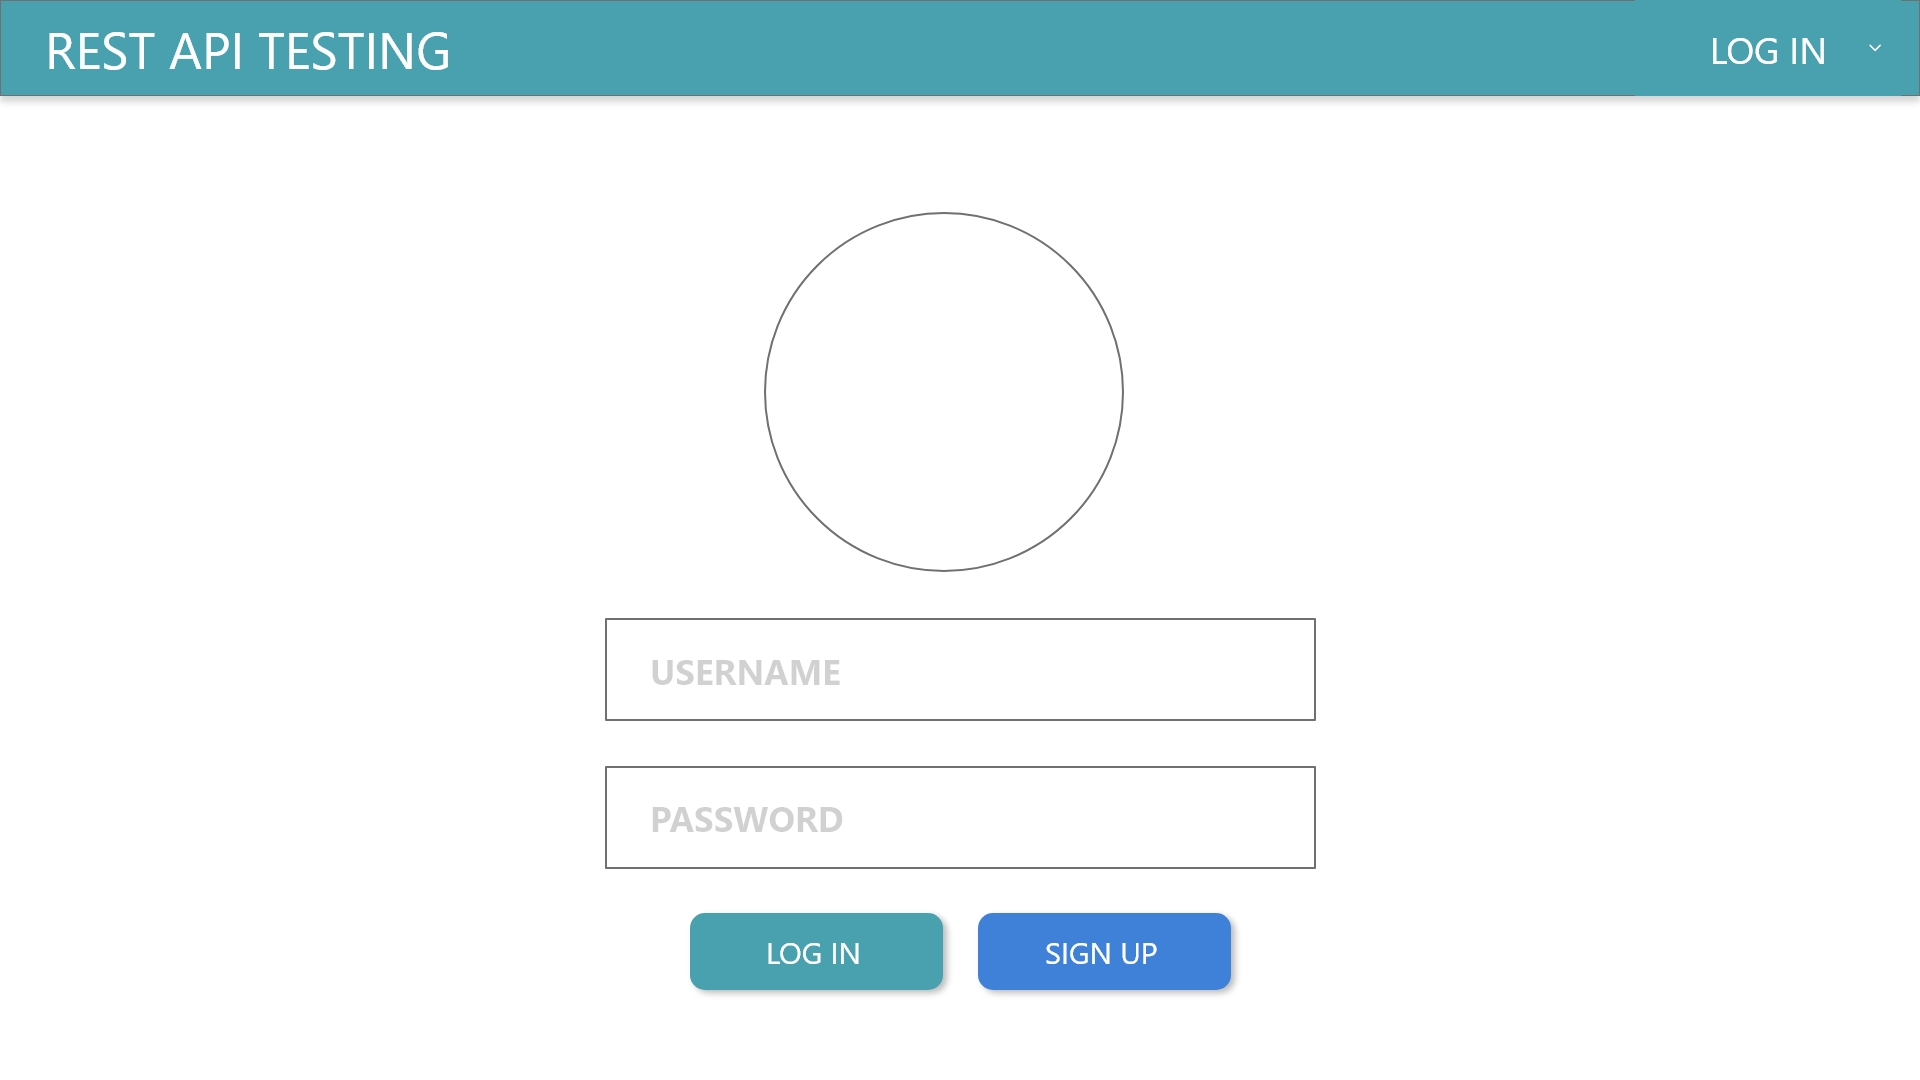
\includegraphics[width=5in]{figures/loginxd.jpg}
	\caption{ตัวอย่างการออกแบบหน้า Log in}
	\label{fig:loginxd}
\end{figure}

\begin{figure}[!thb]
	\captionsetup{justification=centering}
	\centering
	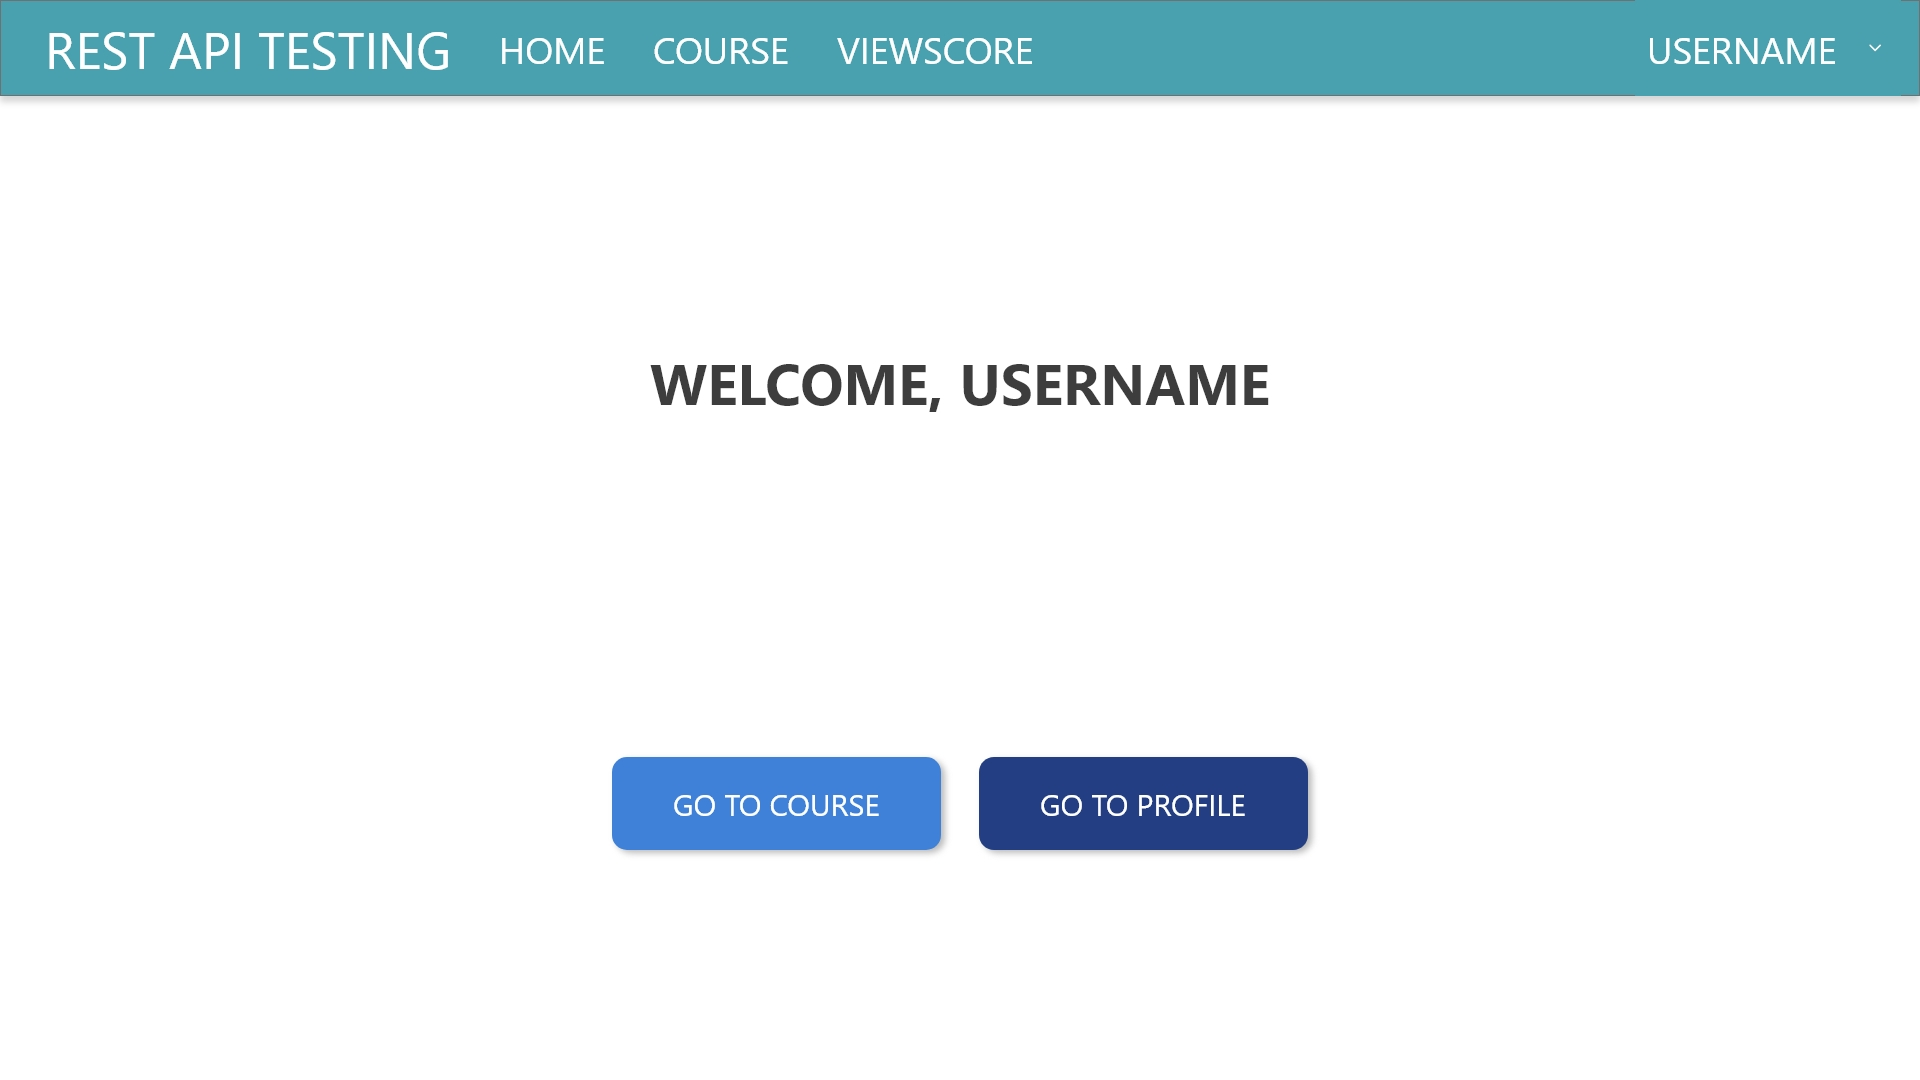
\includegraphics[width=5in]{figures/homepagexd.jpg}
	\caption{ตัวอย่างการออกแบบหน้า Homepage}
	\label{fig:hompagexd}
\end{figure}
\newpage

\begin{figure}[!thb]
	\captionsetup{justification=centering}
	\centering
	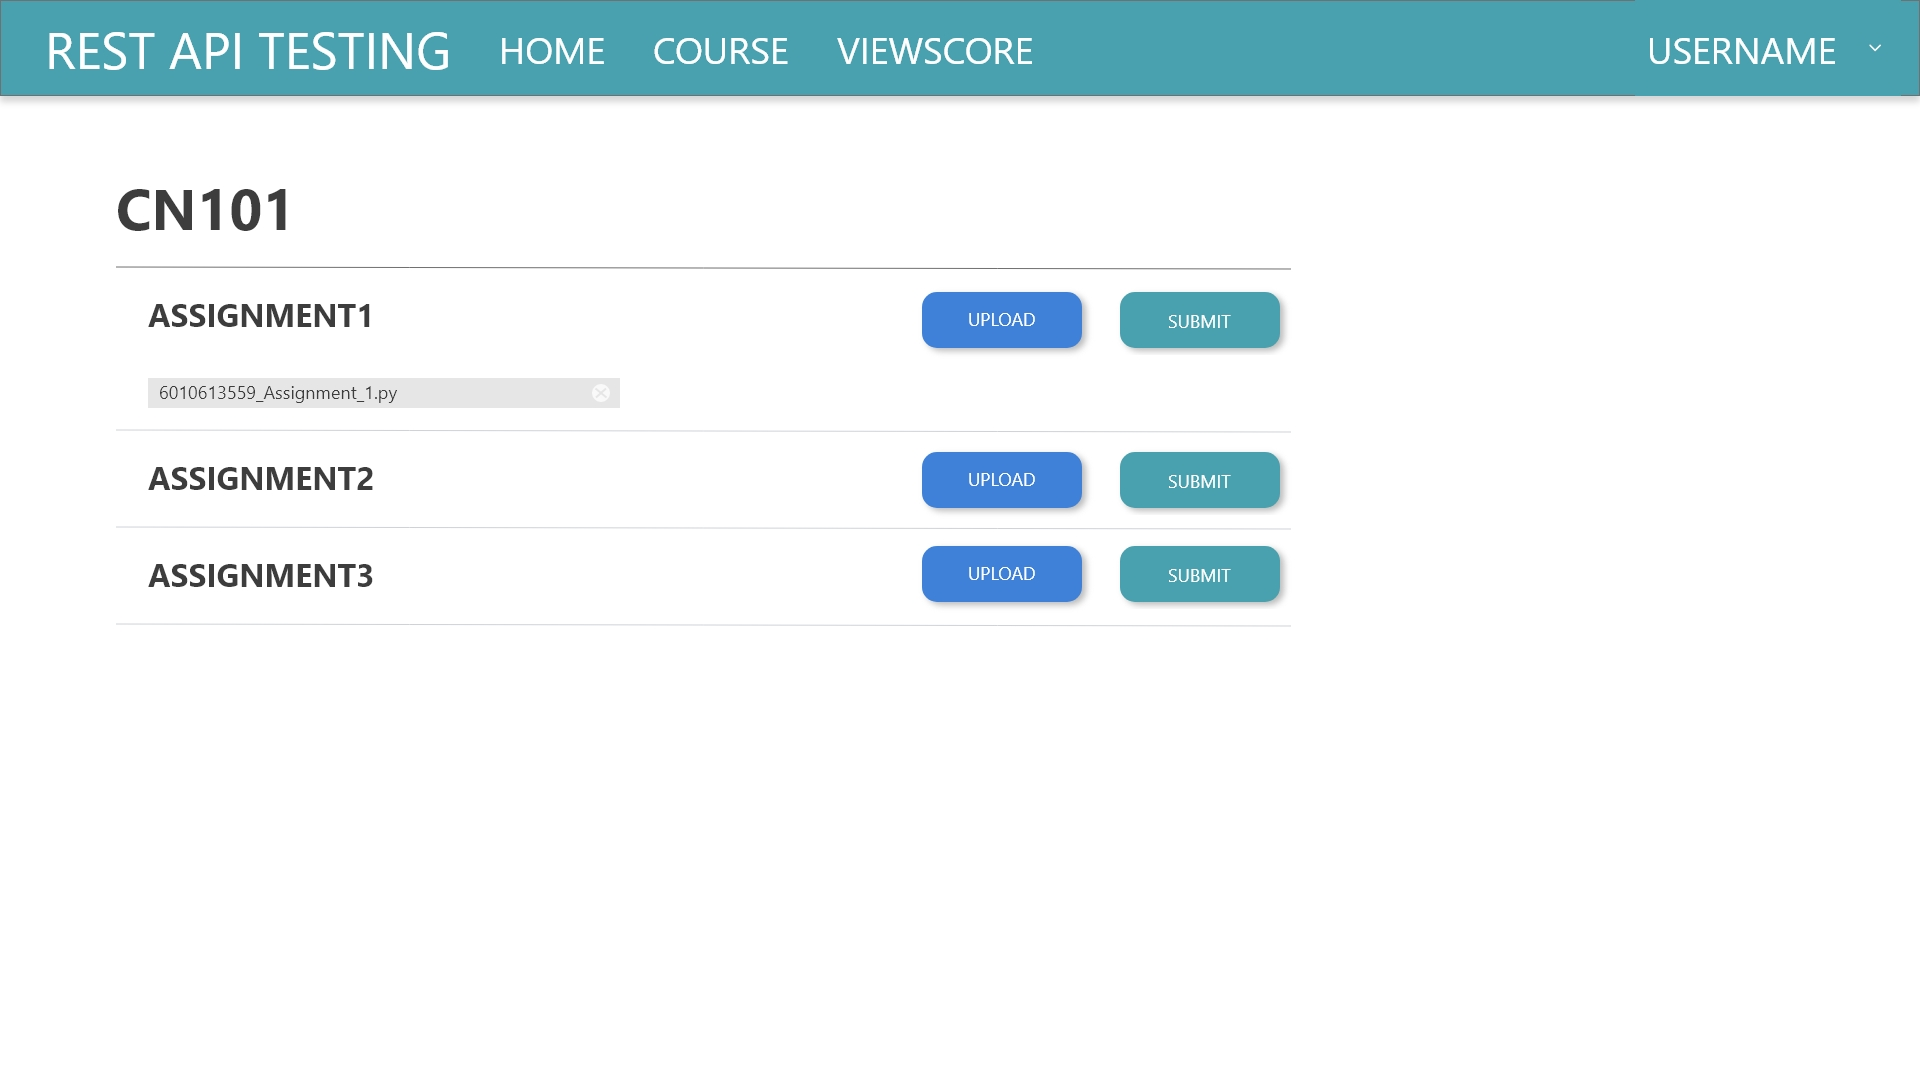
\includegraphics[width=5in]{figures/assignmentxd.jpg}
	\caption{ตัวอย่างการออกแบบหน้า Assignment}
	\label{fig:assignmentxd}
\end{figure}

\begin{figure}[!thb]
	\captionsetup{justification=centering}
	\centering
	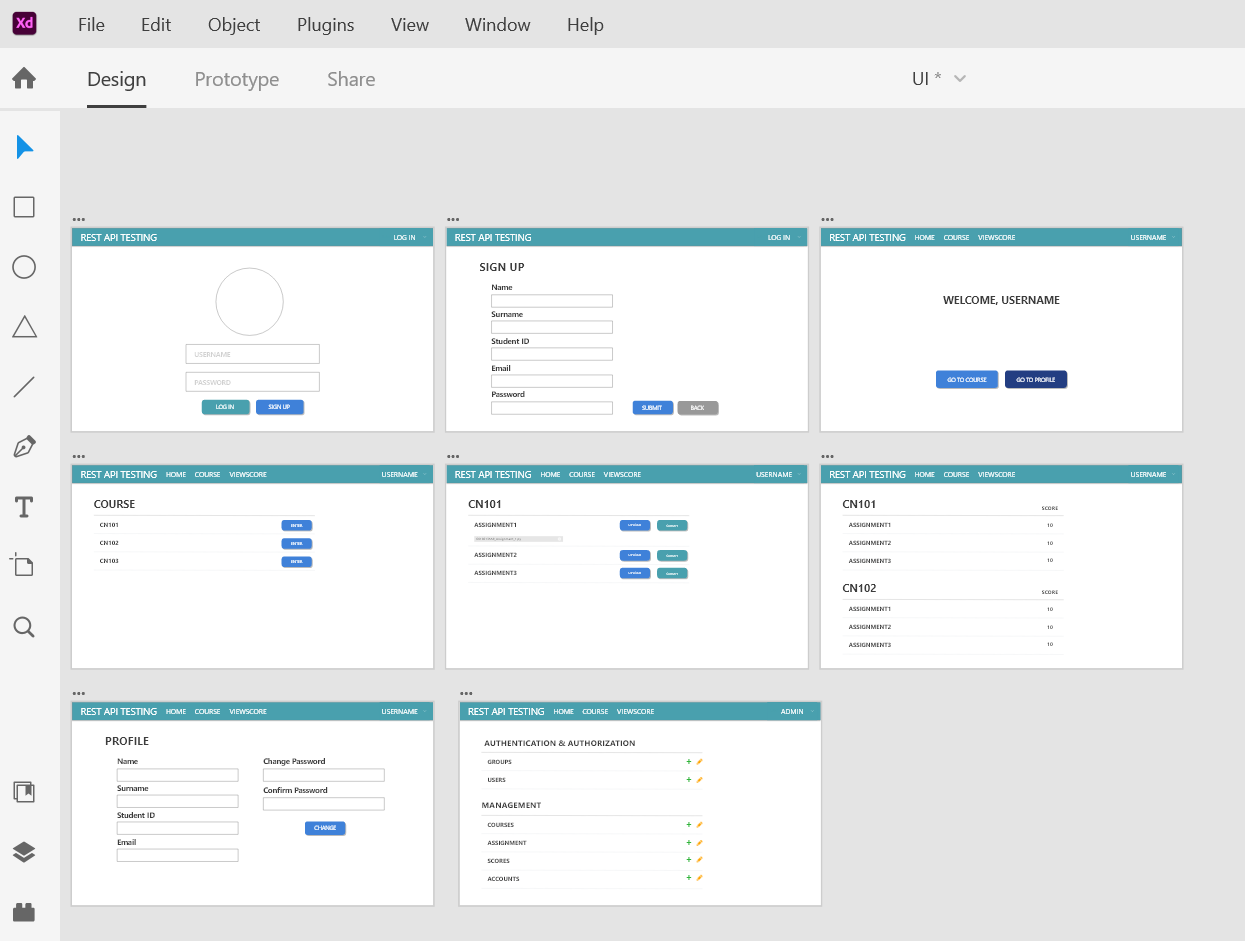
\includegraphics[width=5in]{figures/mockup.png}
	\caption{ตัวอย่างการออกแบบหน้าต่าง ๆ โดยรวม}
	\label{fig:mockup}
\end{figure}
\newpage

\subsection{ภาษาคอมพิวเตอร์}
ภาษาที่เลือกใช้ในการเขียน Website คือภาษา HTML และ Python เนื่องจากภาษา Python มีการใช้งานอย่างแพร่หลาย จึงทำให้ง่ายต่อการเรียนรู้และศึกษา

\subsection{Django Framework}
ในการสร้าง Website ครั้งนี้ได้เลือกใช้ Django Framework เนื่องจาก
ทำงานได้รวดเร็ว มีเครื่องมือให้เลือกใช้ครบ

\subsubsection{การติดตั้ง Django}
หลังจากที่ทำการติดตั้ง Python เรียบร้อยแล้วก่อนจะทำการติดตั้ง Django ได้ทำการติดตั้ง Virtualenv เพื่อแยกสภาพแวดล้อมในการทำงานก่อน 
\begin{itemize}
    \item คำสั่ง pip install virtualenv
    \item และคำสั่ง virtualenv <ชื่อที่ต้องการ>
\end{itemize}
จากนั้นติดตั้ง django ด้วยคำสั่ง 
\begin{itemize}
    \item pip install django ใน virtualenv ที่เราได้ทำการสร้างขึ้น
\end{itemize}
ทำการสร้างโปรเจ็กต์ด้วยคำสั่งและเปิด server 
\begin{itemize}
    \item django-admin startproject <ชื่อโปรเจ็กต์>
    \item python manage.py runserver
\end{itemize}
ทดสอบด้วย http://localhost:8000 ก็จะสามารถเรียก server ขึ้นมาใช้งานได้

\subsubsection{การตั้งค่าการใช้งาน Admin Site}
เนื่องจาก Django Framework มีระบบ Django Administration มาให้สามารถใช้งานอยู่แล้ว จึงสะดวกในการใช้งานมากขึ้น
ในการเปิดใช้งาน Admin Site เริ่มจาก
\begin{itemize}
    \item การสร้าง superuser ด้วยคำสั่ง python manage.py createsuperuser
    \item จากนั้นระบบจะขึ้นให้ตั้งค่า Username และ password
\end{itemize}
เพียงเท่านี้ก็สามารถทำการ Log in ใช้งานหน้าของ Admin Site ได้
\newpage

\begin{figure}[!thb]
	\captionsetup{justification=centering}
	\centering
	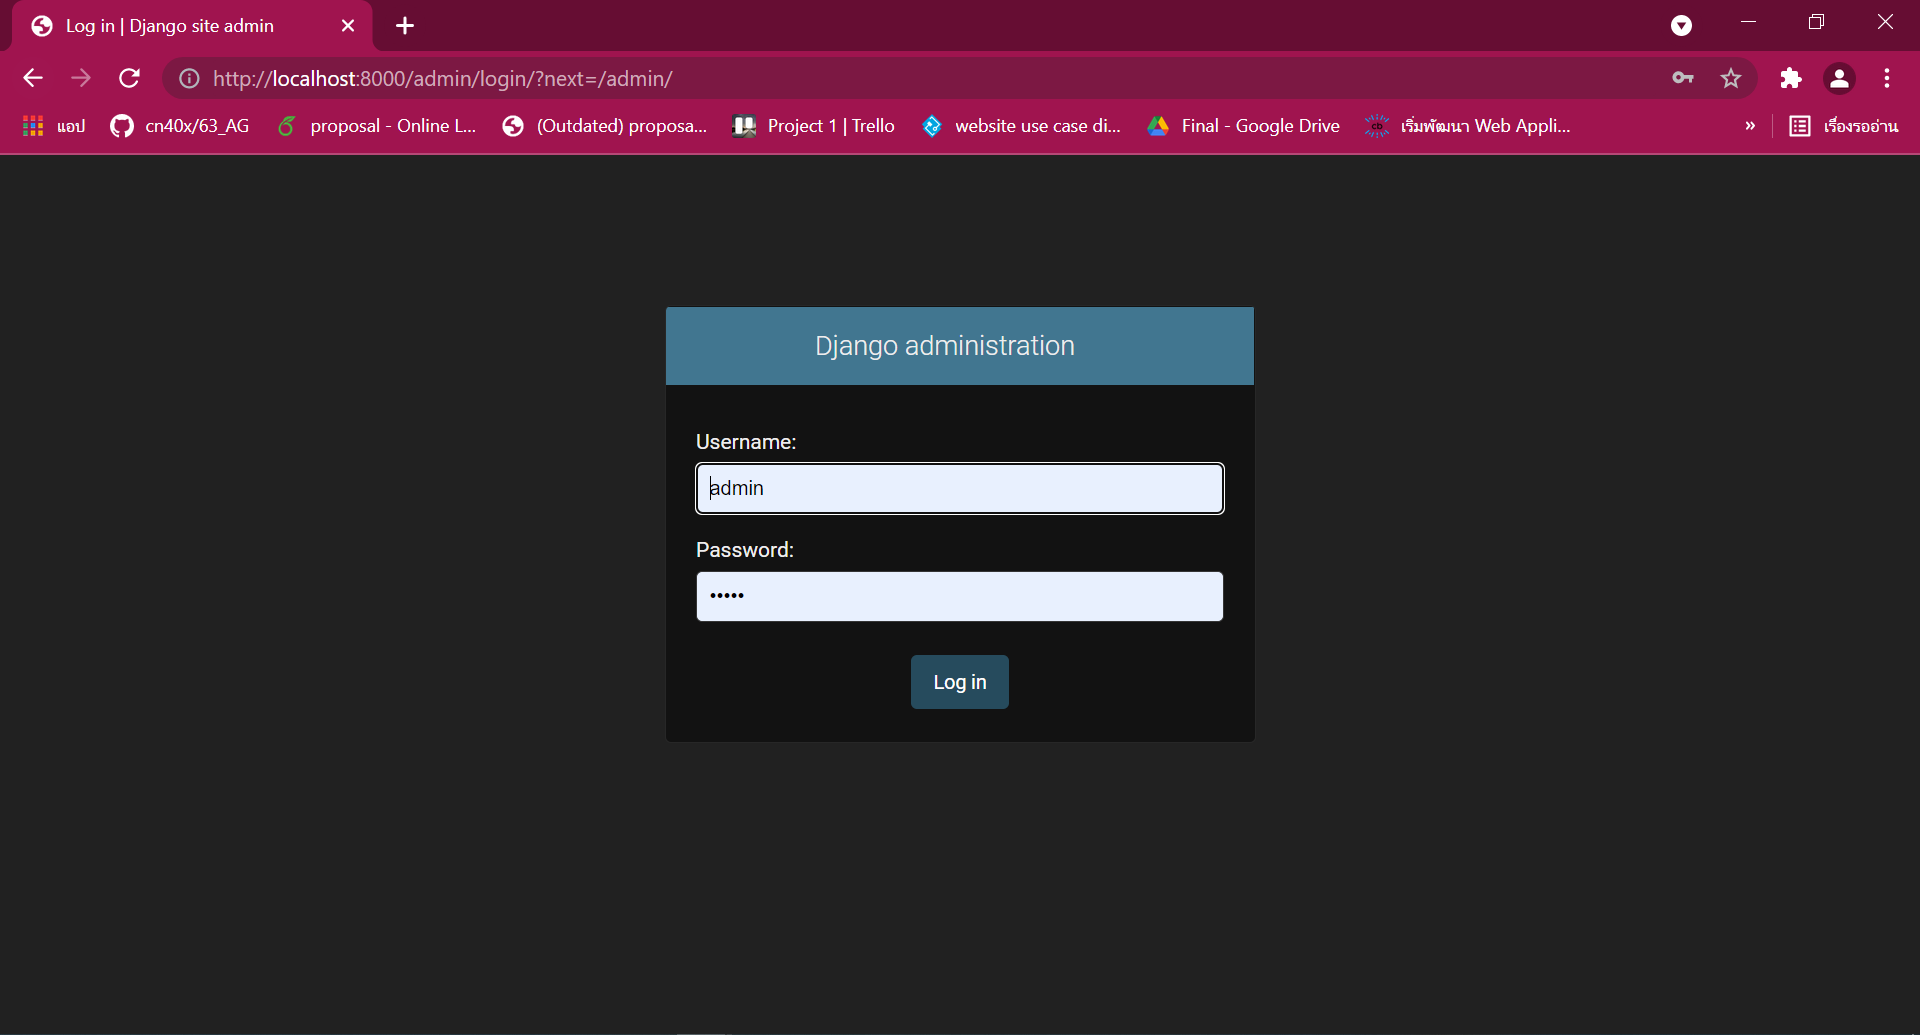
\includegraphics[width=5in]{figures/admin.png}
	\caption{ภาพจากหน้าเว็บ Admin Site}
	\label{figure:admin}
\end{figure}

\begin{figure}[!thb]
	\captionsetup{justification=centering}
	\centering
	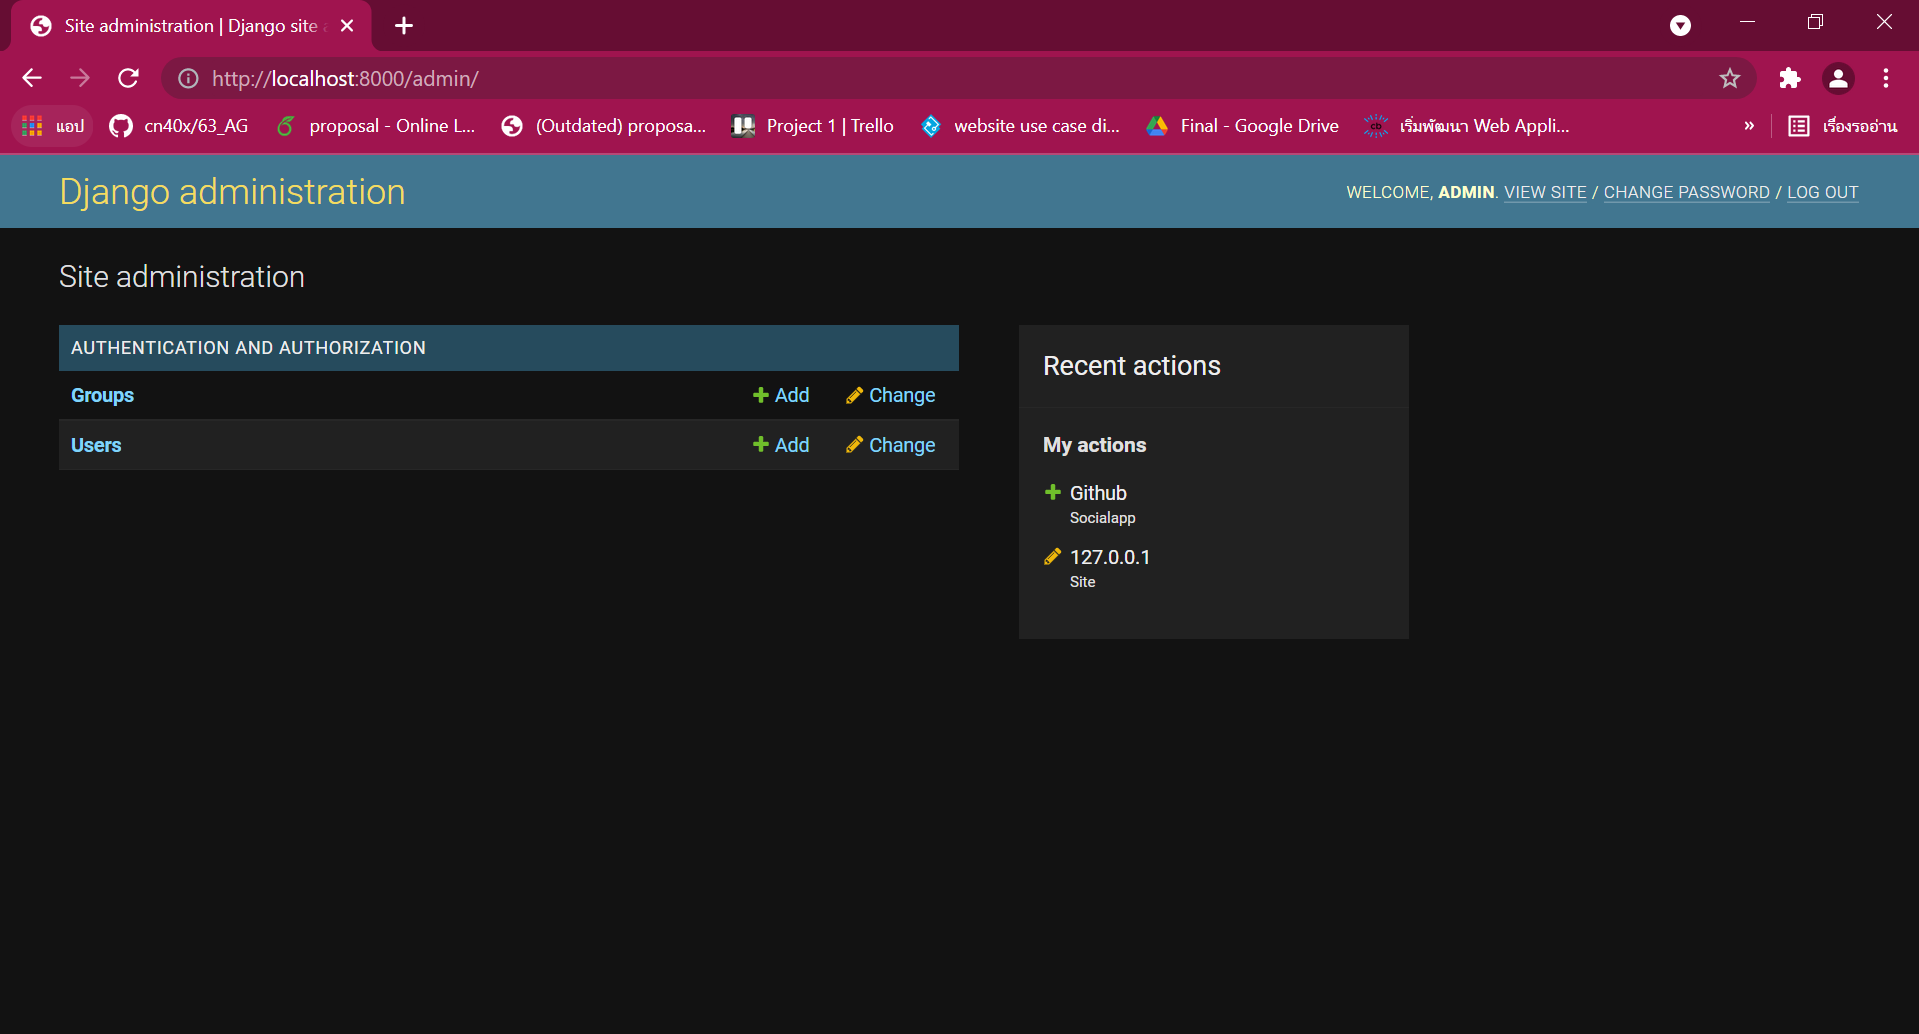
\includegraphics[width=5in]{figures/adminlogin.png}
	\caption{ภาพหน้าเว็บเมื่อทำการ Log in เสร็จสิ้น}
	\label{figure:adminlogin}
\end{figure}
\newpage

\subsection{Website สำหรับใช้งานจริง}
เริ่มต้นการเขียนเว็บด้วยโปรแกรม Virtual Studio Code
โดยรูปแบบการทำงานของ Django จะเป็นแบบ Model View Template (MVT)
\begin{figure}[!thb]
	\captionsetup{justification=centering}
	\centering
	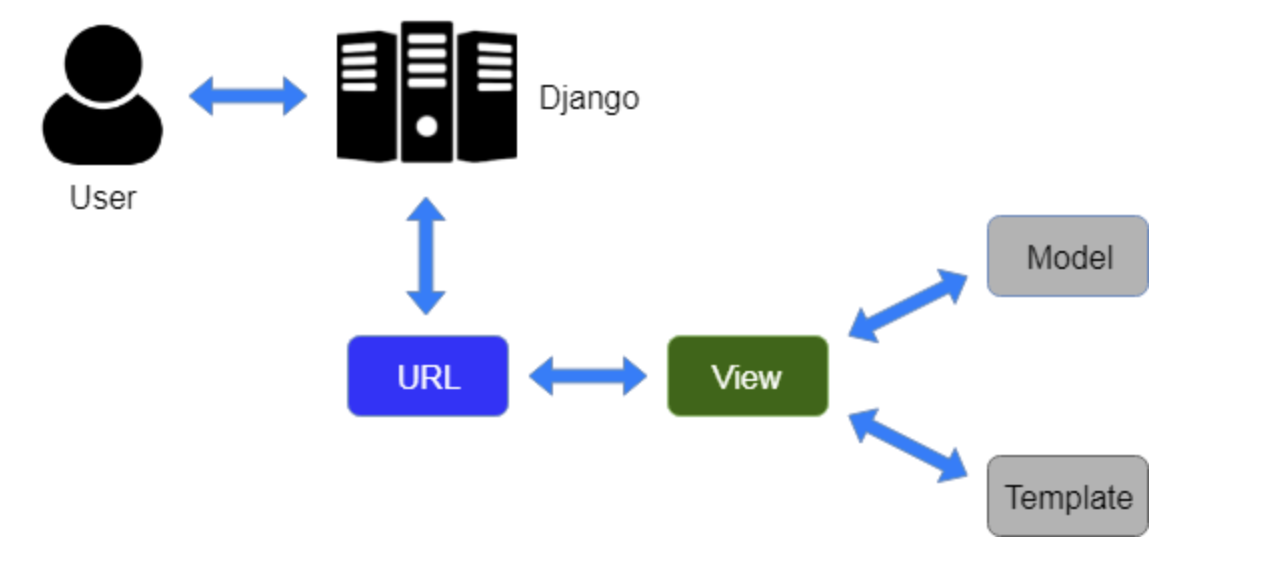
\includegraphics[width=5in]{figures/mvt.png}
	\captionsource{Model-View-Template}{\url{https://www.javatpoint.com/django-mvt}}
	\label{figure:mvt}
\end{figure}

\begin{itemize}
    \item Model คือส่วนที่เก็บข้อมูลของ Application
    \item View สำหรับประมวลผลคำสั่งหรือข้อมูลต่างๆ (เหมือนกับ Controller) และส่งไปแสดงผลตรงส่วนของ Template
    \item Template คือหน้าตา Application ประมวลผลจาก View มาแสดงผลหน้าเว็บร่วมกับ HTML
\end{itemize}

\newpage
หลังจากที่ทำการ startproject ไปในขั้นตอนของการติดตั้งเรียบร้อยแล้ว โครงสร้างของโปรเจ็กต์จะเป็นรูปแบบดังนี้

\begin{figure}[!thb]
	\captionsetup{justification=centering}
	\centering
	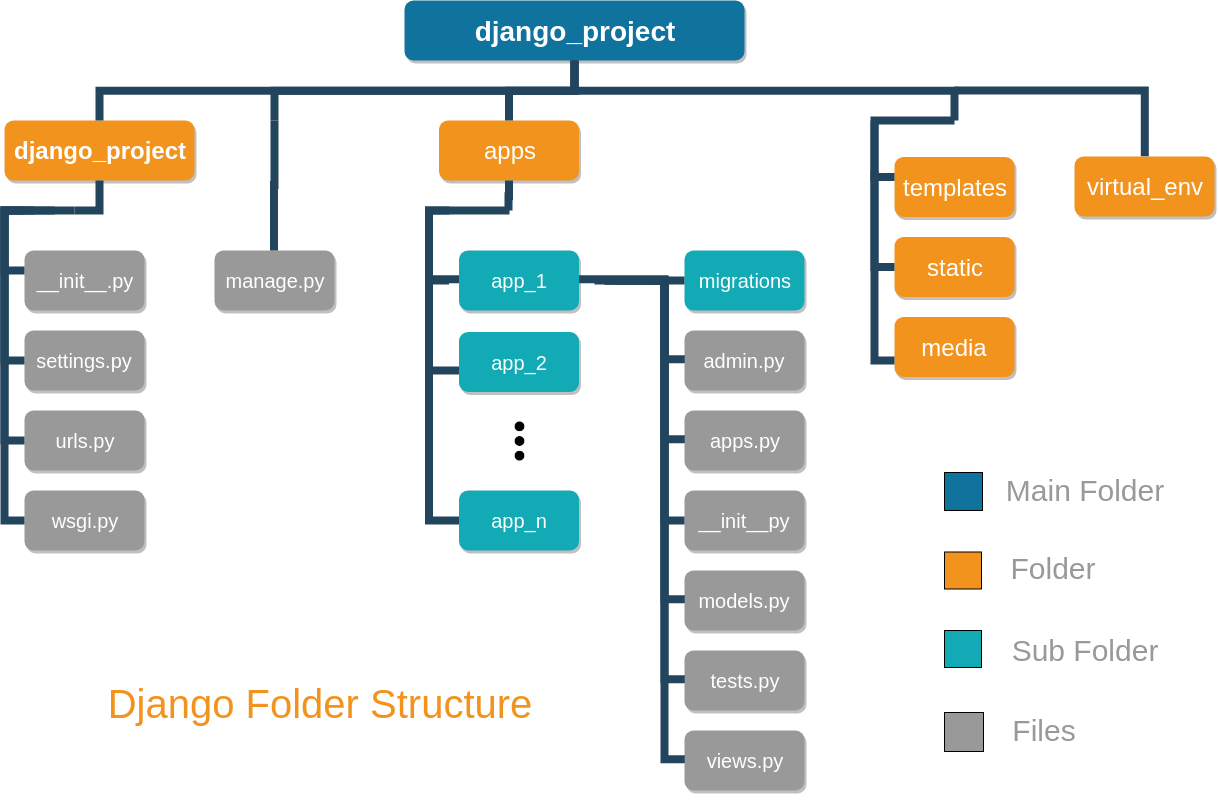
\includegraphics[width=6in]{figures/djangoproject.png}
	\captionsource{Django Project Structure}{\url{https://studygyaan.com/django/best-practice-to-structure-django-project-directories-and-files}}
	\label{fig:djangoproject}
\end{figure}
\newpage

ในการดำเนินงานเบื้องต้นได้ทำการเขียนเว็บในส่วนของ template หน้าต่างๆ  สามารถเชื่อมต่อหากันในแต่ละหน้าได้ และ สามารถ Runserver ขึ้นมาเพื่อใช้งานได้ดังนี้

\begin{figure}[!thb]
	\captionsetup{justification=centering}
	\centering
	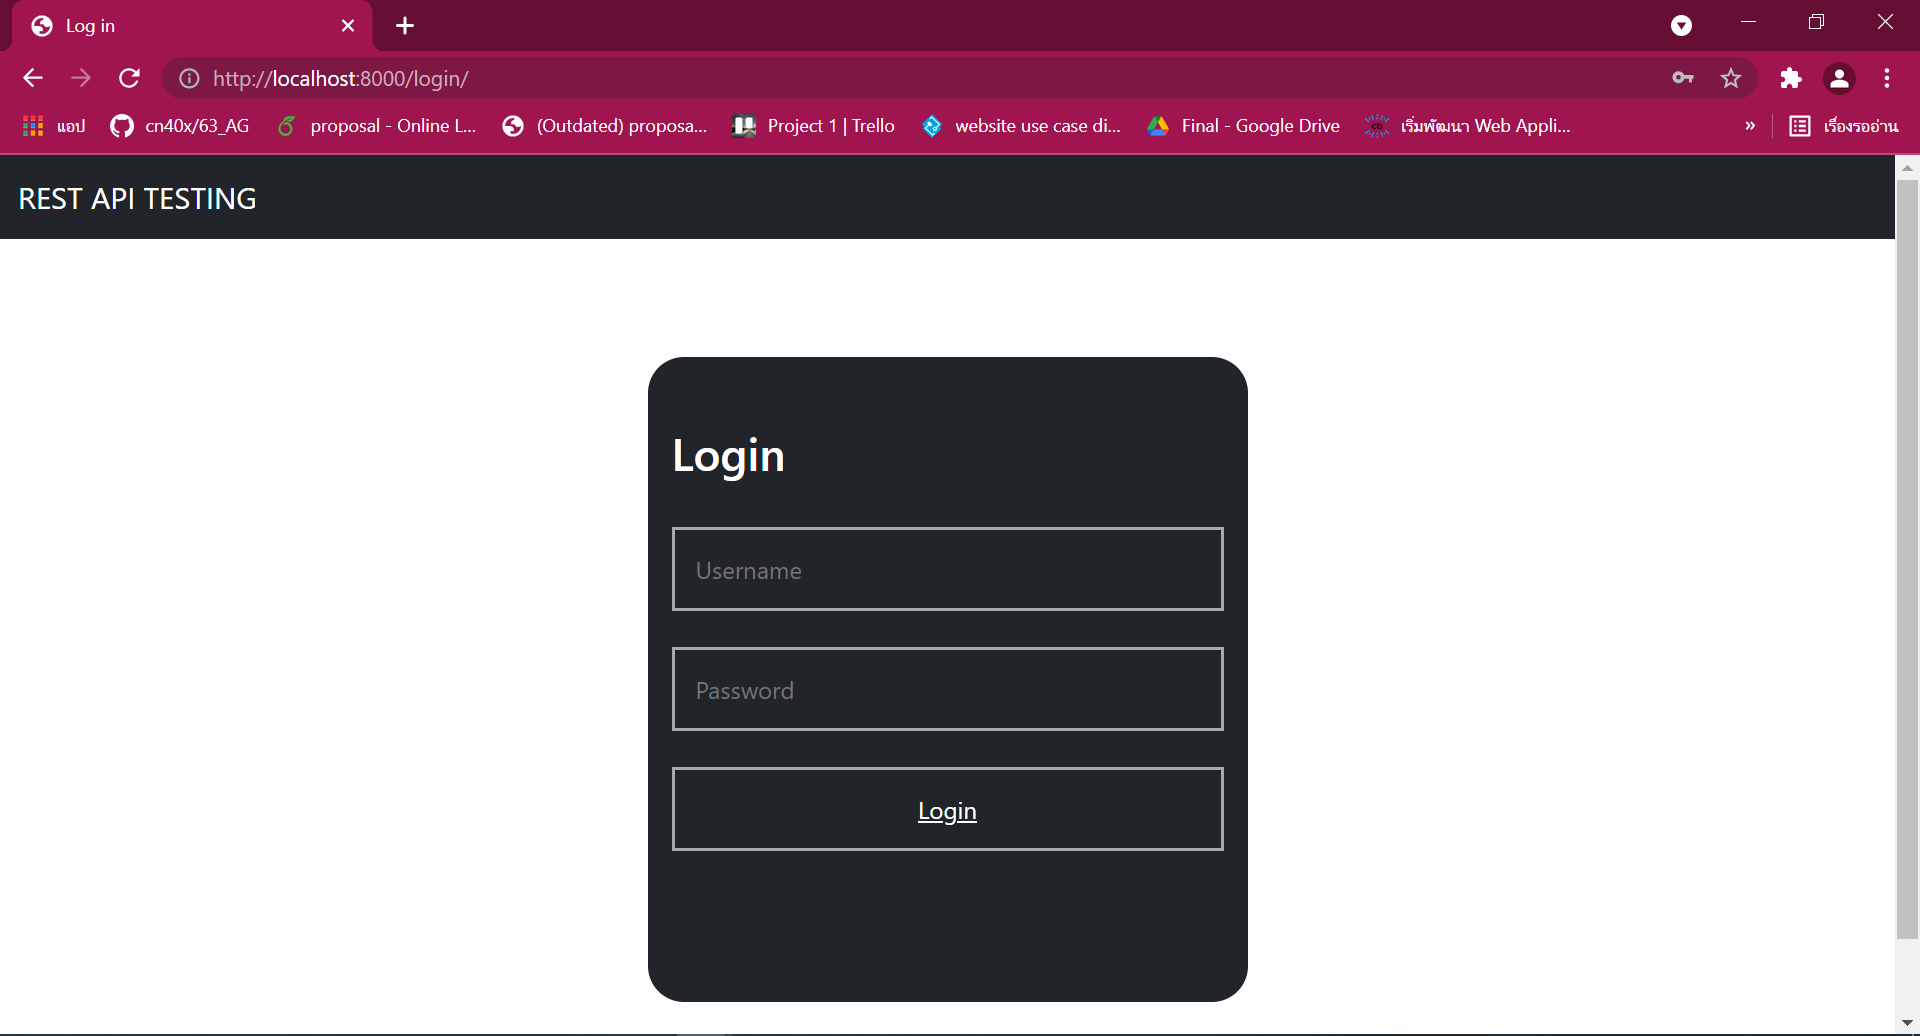
\includegraphics[width=5in]{figures/login.png}
	\caption{รูปภาพในส่วนของหน้า Log in}
	\label{fig:login}
\end{figure}
\noindent จากรูปที่ \ref{fig:login} แสดงการเข้าถึงเว็บด้วยการ Log in ในส่วนนี้ยังไม่สามารถทำการ Log in ได้จริง ๆ เนื่องจากยังอยู่ในระหว่างการศึกษาเพื่อจะนำการ Authentication มาใช้ร่วม
\newline
\begin{figure}[!thb]
	\captionsetup{justification=centering}
	\centering
	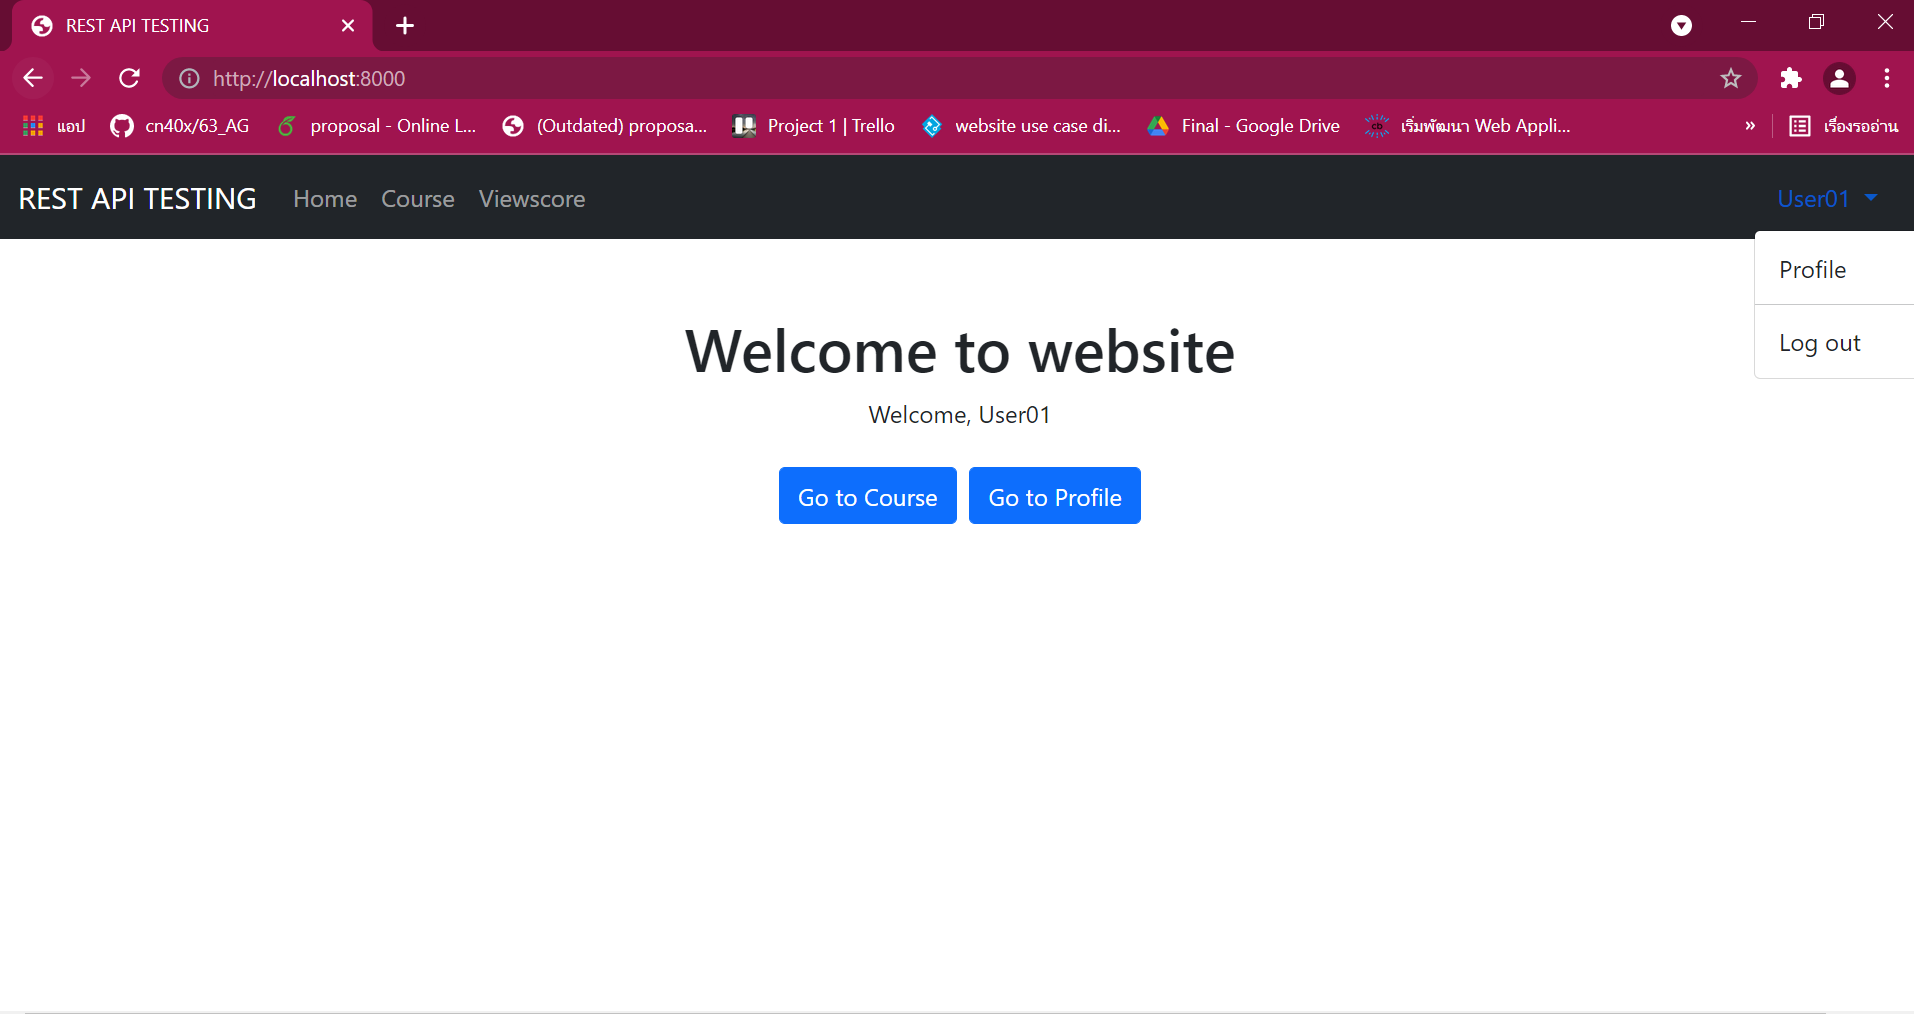
\includegraphics[width=5in]{figures/home.png}
	\caption{รูปภาพในส่วนของหน้า Home}
	\label{fig:home}
\end{figure}
\newline
จากรูปที่ \ref{fig:home} เมื่อ Log in เข้ามาแล้วจะเจอกับหน้าหลักหรือหน้า Home ของเว็บ จากหน้านี้สามารถเข้าถึงหรือเชื่อมต่อไปยังหน้า template อื่น ๆ ได้
\newpage

\begin{figure}[!thb]
	\captionsetup{justification=centering}
	\centering
	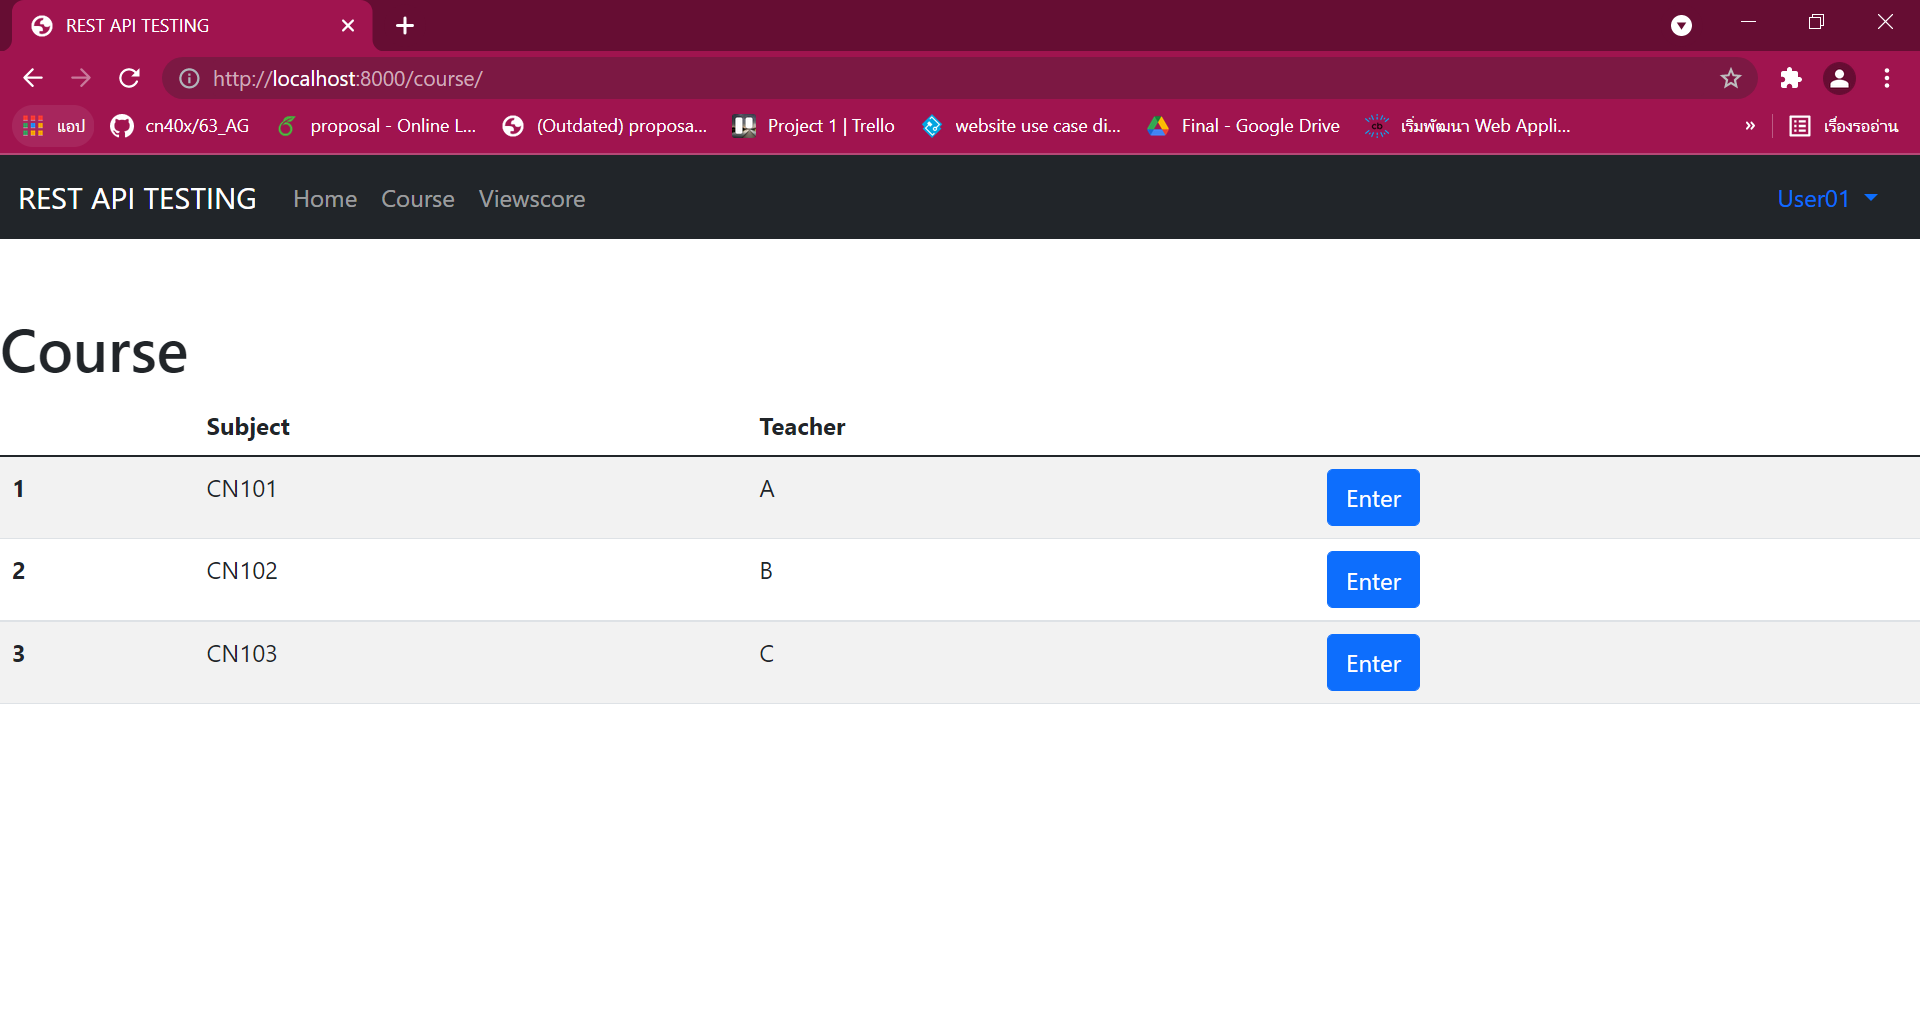
\includegraphics[width=5in]{figures/course.png}
	\caption{รูปภาพในส่วนของหน้า Course}
	\label{fig:coure}
\end{figure}
\noindent จากรูปที่ \ref{fig:coure} ในหน้า Course หรือ
วิชาเรียนสามารถกดปุ่ม Enter เพื่อไปยังหน้า Assignment

\begin{figure}[!thb]
	\captionsetup{justification=centering}
	\centering
	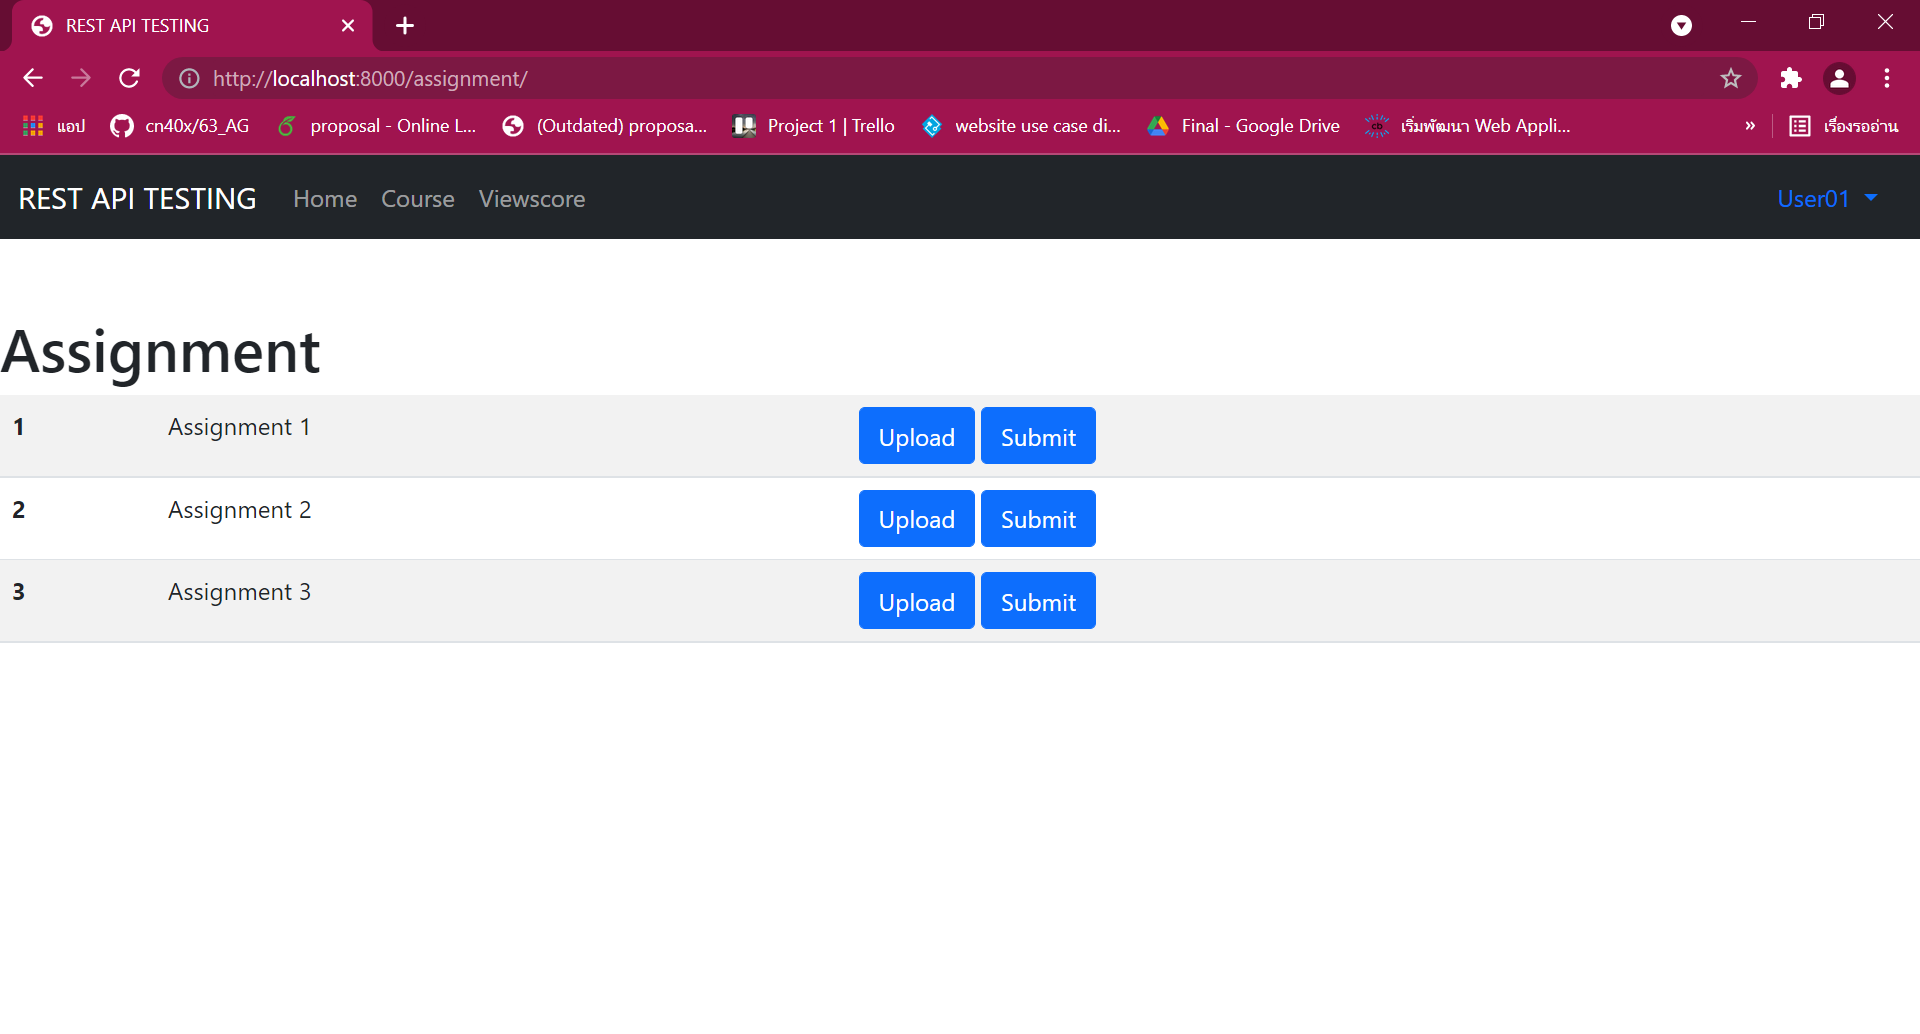
\includegraphics[width=5in]{figures/assign.png}
	\caption{รูปภาพในส่วนของหน้า Assignment}
	\label{fig:assign}
\end{figure}
\noindent จากรูปที่ \ref{fig:assign} หน้า Assignment แสดงการบ้านต่าง ๆ สามารถกดปุ่ม upload เพื่อเลือกไฟล์จากเครื่องได้ ในส่วนนี้ยังไม่สามารถ upload ได้จริงเนื่องจากยังไม่มีฐานข้อมูลให้เก็บ และสามารถกดปุ่ม submit เพื่อไปยังหน้าของ Viewscore ได้
\newpage

\begin{figure}[!thb]
	\captionsetup{justification=centering}
	\centering
	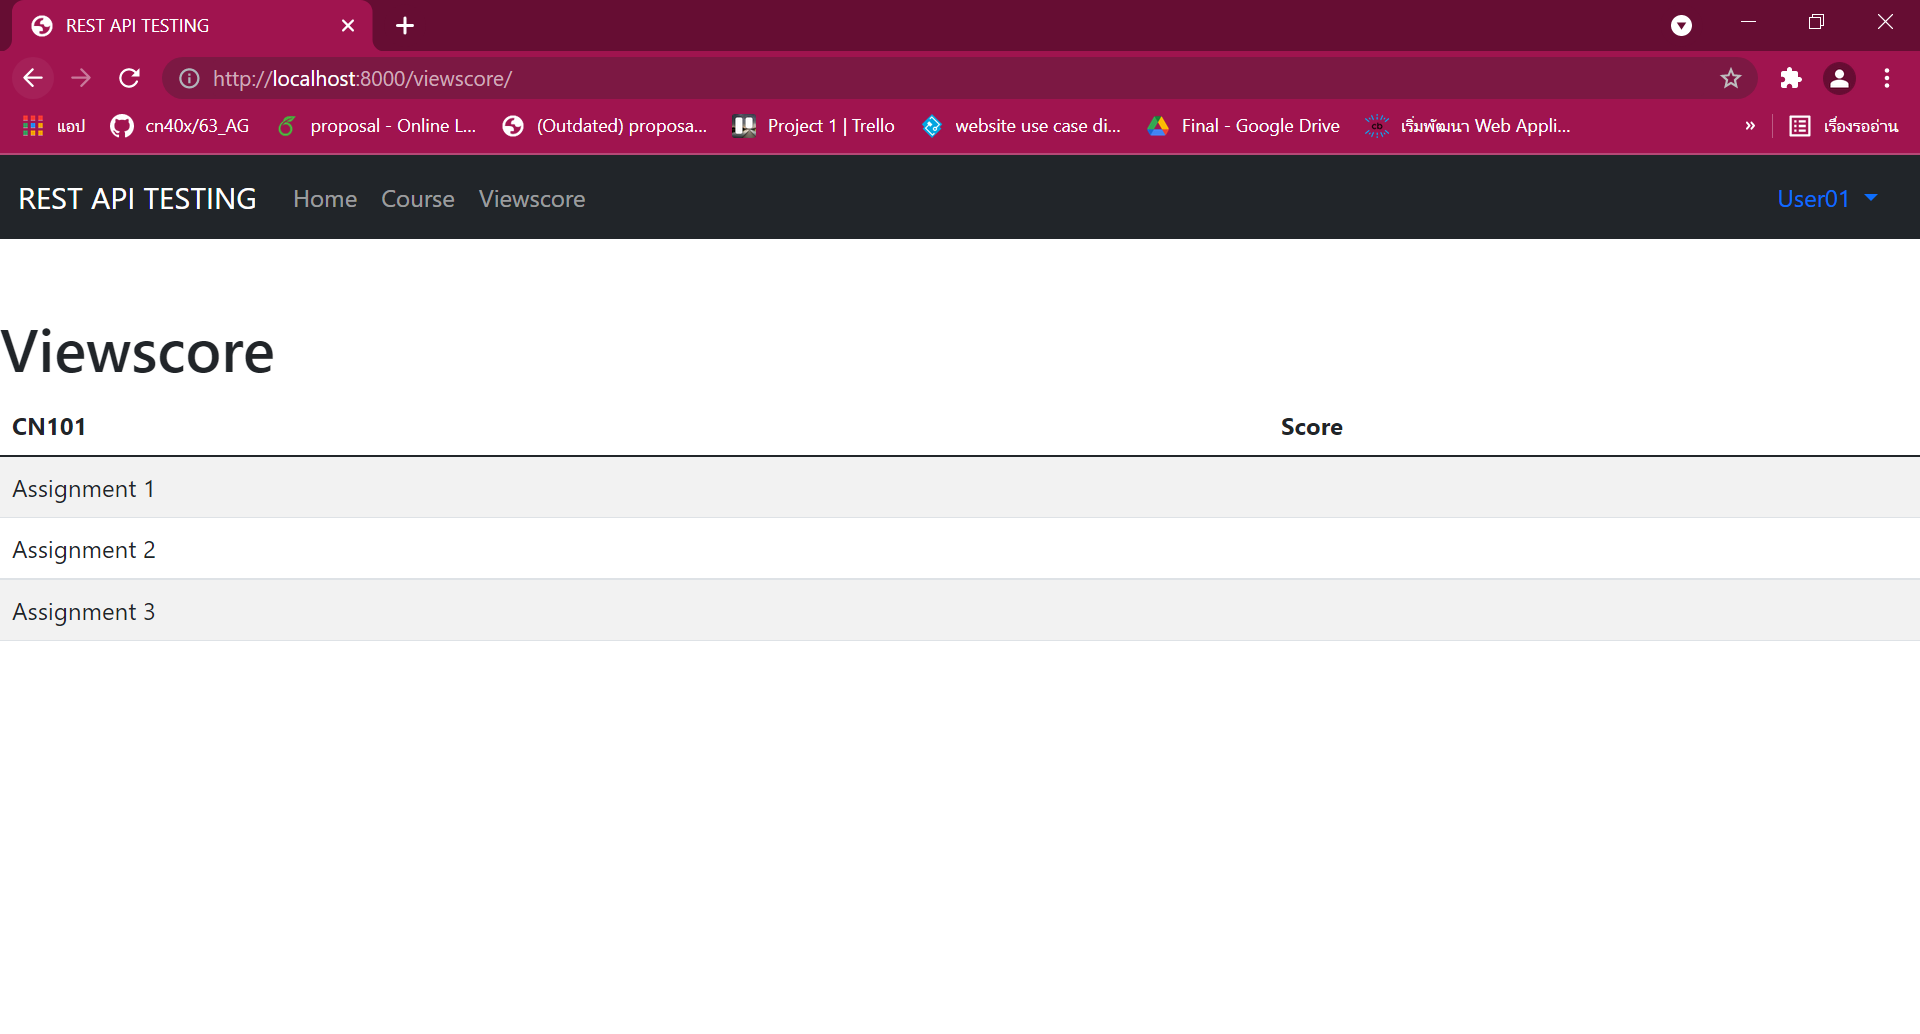
\includegraphics[width=5in]{figures/score.png}
	\caption{รูปภาพในส่วนของหน้า View Score}
	\label{fig:score}
\end{figure}
\noindent จากรูปที่ \ref{fig:score} หน้า Viewscore จะเป็นหน้าที่ใช้ในการแสดงผลคะแนนของแต่ละ\mbox{การบ้าน}
\begin{figure}[!thb]
	\captionsetup{justification=centering}
	\centering
	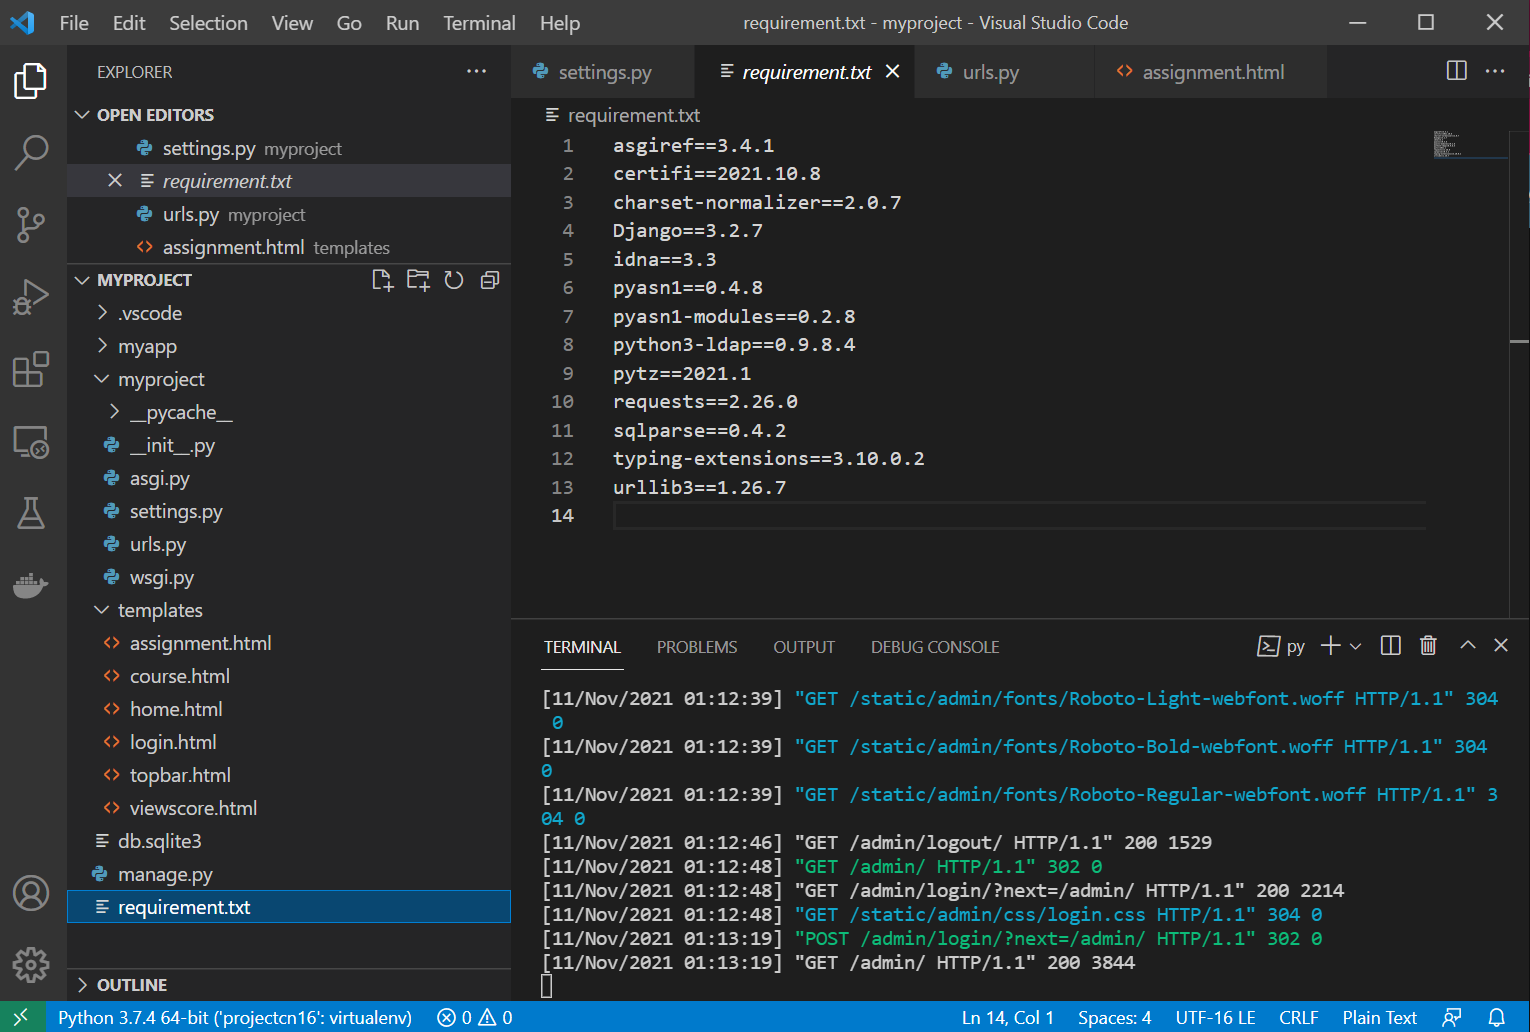
\includegraphics[width=5in]{figures/code.png}
	\caption{แสดงโปรแกรมใน requirement.txt}
	\label{fig:code}
\end{figure}
\newline
จากรูปที่ \ref{fig:code} แสดงการติดตั้งโปรแกรมทั้งหมด ณ ปัจจุบันอยู่ในไฟล์ requirement.txt
\newpage

\section{ศึกษาการทำ Authentication ในการ Login }
โดยทั่วไปการใช้เว็บไซต์ แพลทฟอร์ม หรือ social media ต่าง ๆ ในโลกอินเตอร์เน็ต\mbox{จำเป็น}จะต้องมีการ Login เพื่อเข้าใช้งานและจะต้องมีการระบุตัวตนว่าผู้ใช้งานคนนี้เป็นใคร ด้วยการ Authentication

\subsection{Authentication คืออะไร}
Authentication คือ ระบบการยืนยันตัวตนที่เมื่อเราจะเข้าใช้งานในเว็บไซต์ \mbox{แอปพลิเคชัน}หรืออะไรก็ตามบนโลกออนไลน์เพื่อใช้ในการ Login
เราจะต้องสามารถยืนยันตัวตนได้โดยปกติจะใช้การยืนยันตัวตนจาก username และ password
\begin{figure}[!thb]
	\captionsetup{justification=centering}
	\centering
	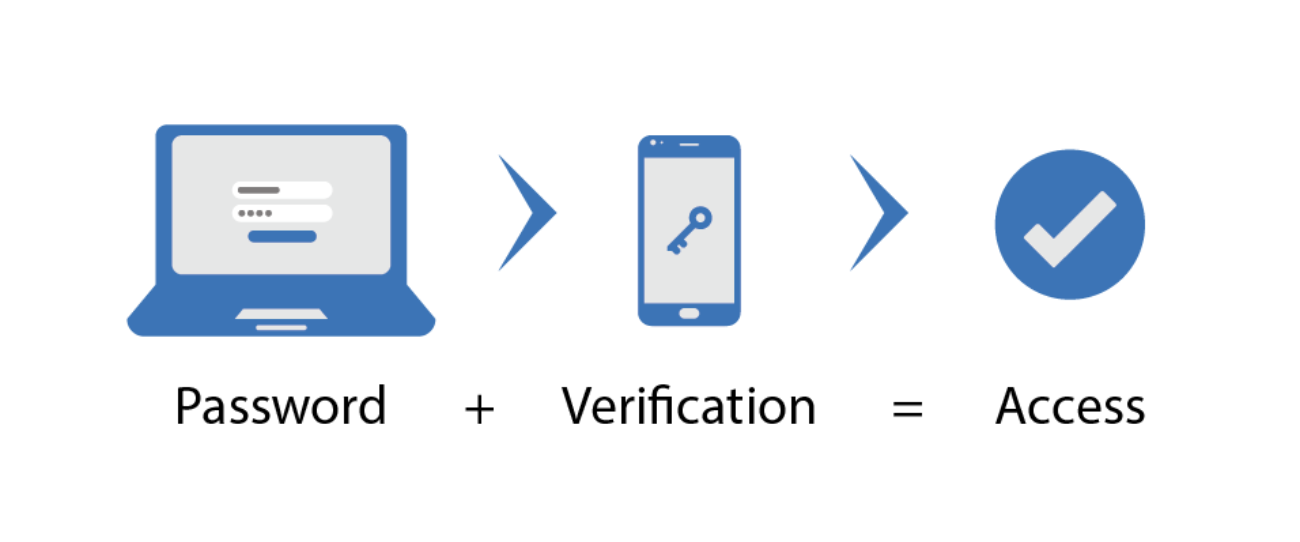
\includegraphics[width=6in]{figures/authen.png}
	\captionsource{Authentication}{\url{https://medium.com/ingrammicroth/}}
	\label{fig:authen}
\end{figure}
\newpage

\subsection{Authentication โดยใช้ LDAP }
หน่วยงานจะจัดเก็บชื่อผู้ใช้ รหัสผ่าน ที่อยู่อีเมล และข้อมูลคงที่อื่นๆ ภายใน directory LDAP เป็นโปรโตคอลแอปพลิเคชันแบบเปิดและเป็นกลางสำหรับการเข้าถึงและบำรุงรักษาข้อมูลนั้น LDAP ยังสามารถจัดการกับการตรวจสอบสิทธิ์ ดังนั้นผู้ใช้สามารถลงชื่อเข้าใช้เพียงครั้งเดียวและเข้าถึงไฟล์ต่างๆ มากมายบนเซิร์ฟเวอร์ เนื่องจาก LDAP เป็นโปรโตคอล จึงไม่ระบุวิธีการทำงานของโปรแกรม directory แต่เป็นรูปแบบของภาษาที่ช่วยให้ผู้ใช้สามารถค้นหาข้อมูลที่ต้องการได้อย่างรวดเร็ว
\begin{flushleft}
	\textbf{ข้อดีของ LDAP}
\end{flushleft}
\begin{itemize}
    \item LDAP เก็บข้อมูลเป็นโครงสร้างแบบต้นไม้ ซึ่งสามารถเก็บข้อมูลแยกกันอยู่หลาย ๆ เครื่องได้โดยแยกตามโครงสร้างของต้นไม้
    \item LDAP สามารถทำงานได้ทั้งบนโปรโตคอลแบบ Secure และไม่ Secure
    \item ระบบ Authentication บน Linux สามารถใช้งานผ่าน LDAP ได้อย่างสมบูรณ์
    \item สามารถทำ Replication ได้
\end{itemize}


\begin{figure}[!thb]
	\captionsetup{justification=centering}
	\centering
	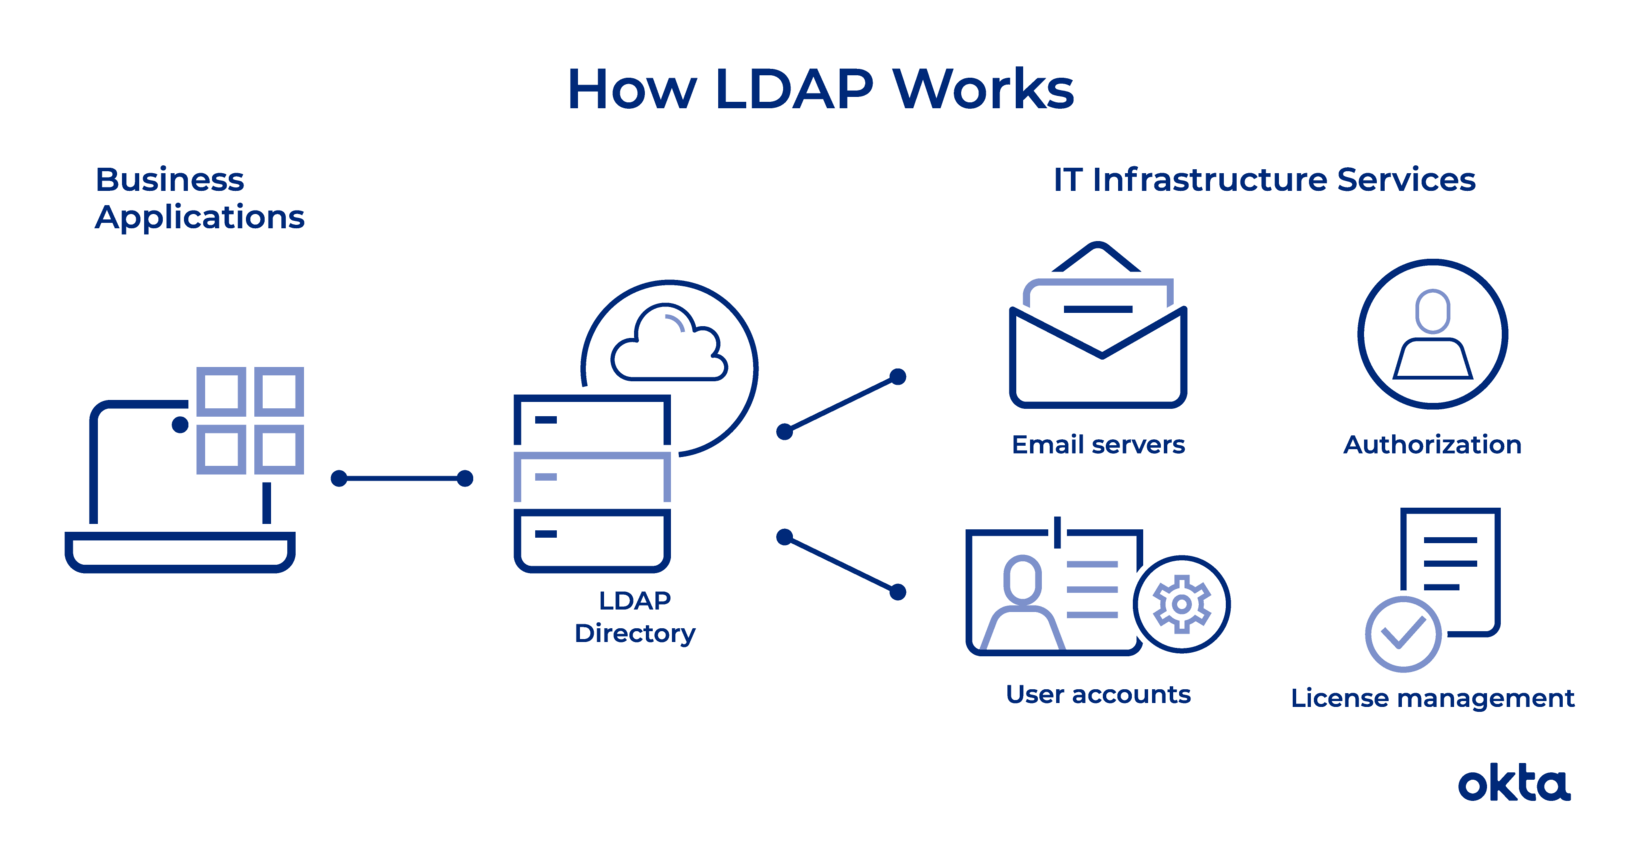
\includegraphics[width=6in]{figures/ldap.png}
	\captionsource{LDAP Authentication}{\url{https://www.okta.com/identity-101/what-is-ldap/}}
	\label{fig:ldap}
\end{figure}
\newpage

\subsubsection{โครงสร้างของ LDAP Directory}
ตัว entry (ตำแหน่งข้อมูล) จะประกอบด้วยชุดของ attributes ทุก attribute จะมีชื่อ (type, description) ซึ่งจะกำหนดใน schema ทุก entry ต้องไม่ซ้ำกัน ซึ่งเป็น Distinguished Name (DN) cn คือ Common Name และ dc คือ Domain Component Server จะเก็บข้อมูลในลักษณะ subtree โดยจะเริ่มหาทีละ entry เช่น “dc=example,dc=com” โดย server อาจจะใช้ server อื่นเป็นตัวอ้างอิง เช่น “ou=department,dc=example,dc=com” อาจจะตอบกลับมาเป็น reference ไปที่ server ที่มีข้อมูลอยู่ในส่วนของ directory tree ซึ่งทาง client สามารถที่จะติดต่อกับ server อื่นได้
\begin{figure}[!thb]
    \captionsetup{justification=centering}
    \centering
    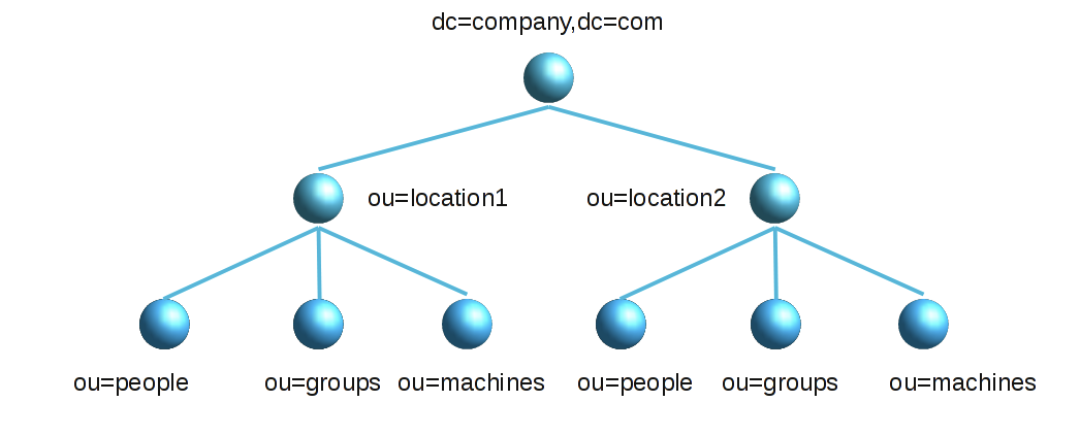
\includegraphics[width=5in]{figures/ldap-structure.png}
    \captionsource{LDAP Structure}{\url{https://saixiii.com/what-is-ldap/}}
    \label{fig:ldap-structure}
\end{figure}
\newpage

\subsubsection{ตัวอย่างองค์ประกอบการ Coding ของ LDAP}
\begin{figure}[!thb]
\captionsetup{justification=centering}
\centering
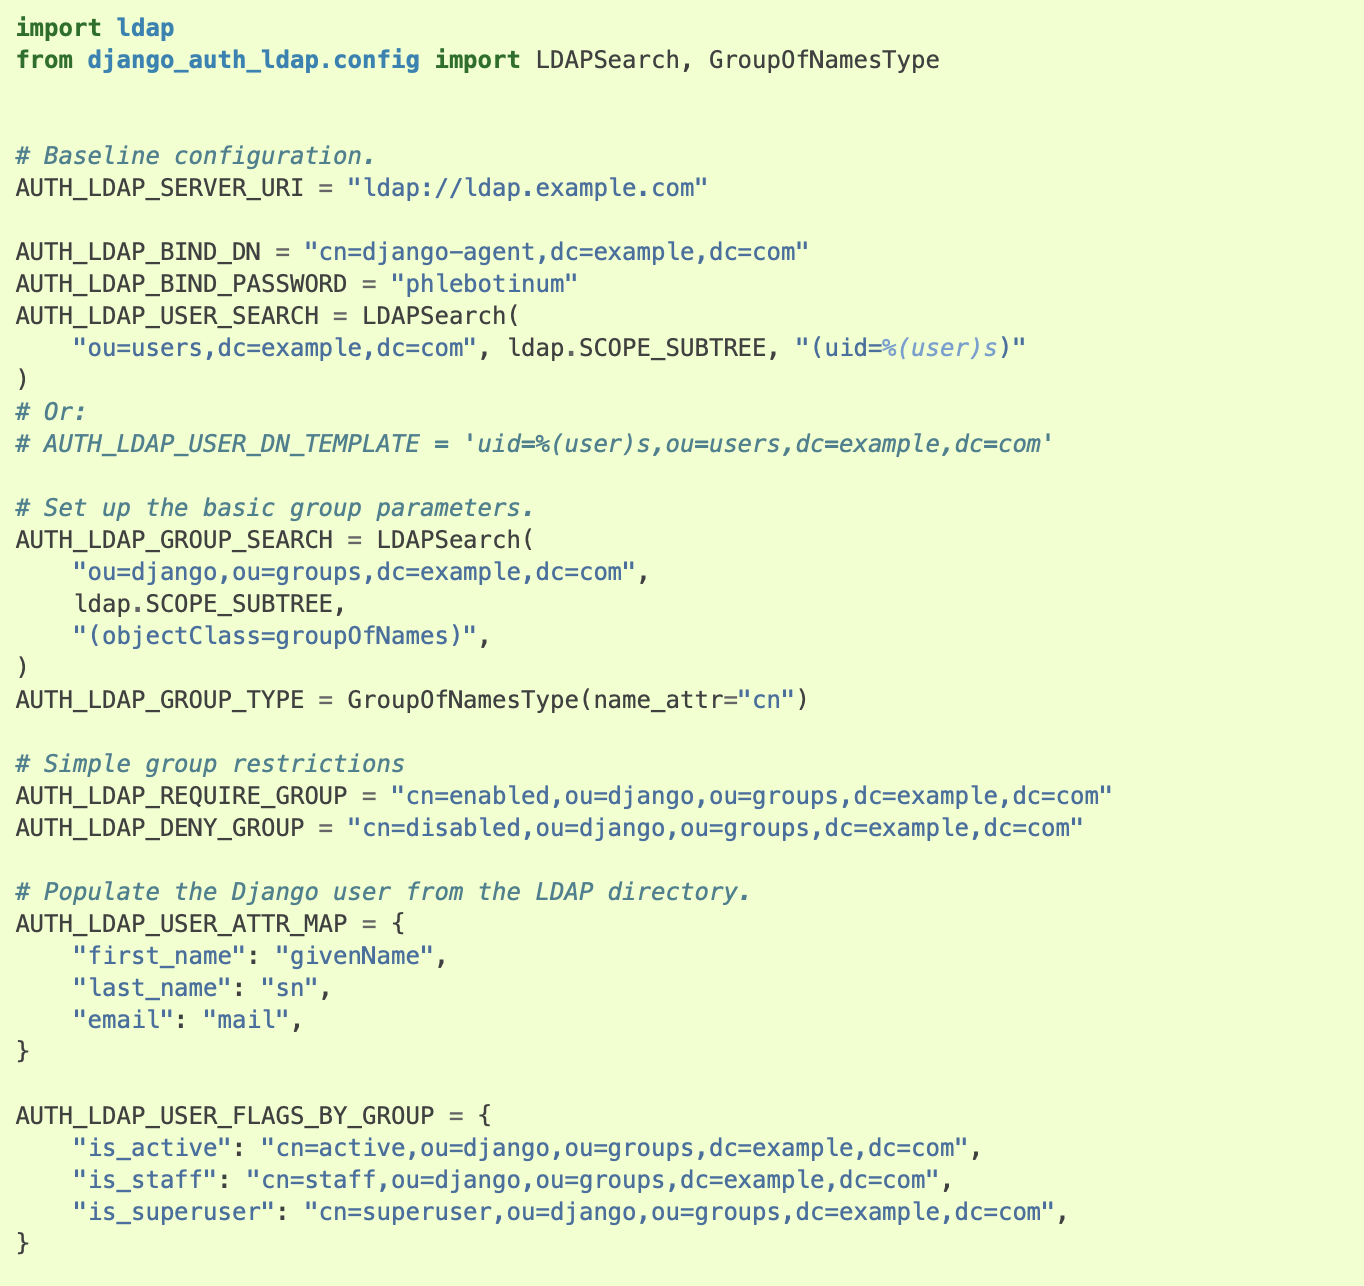
\includegraphics[width=6in]{figures/exam1}
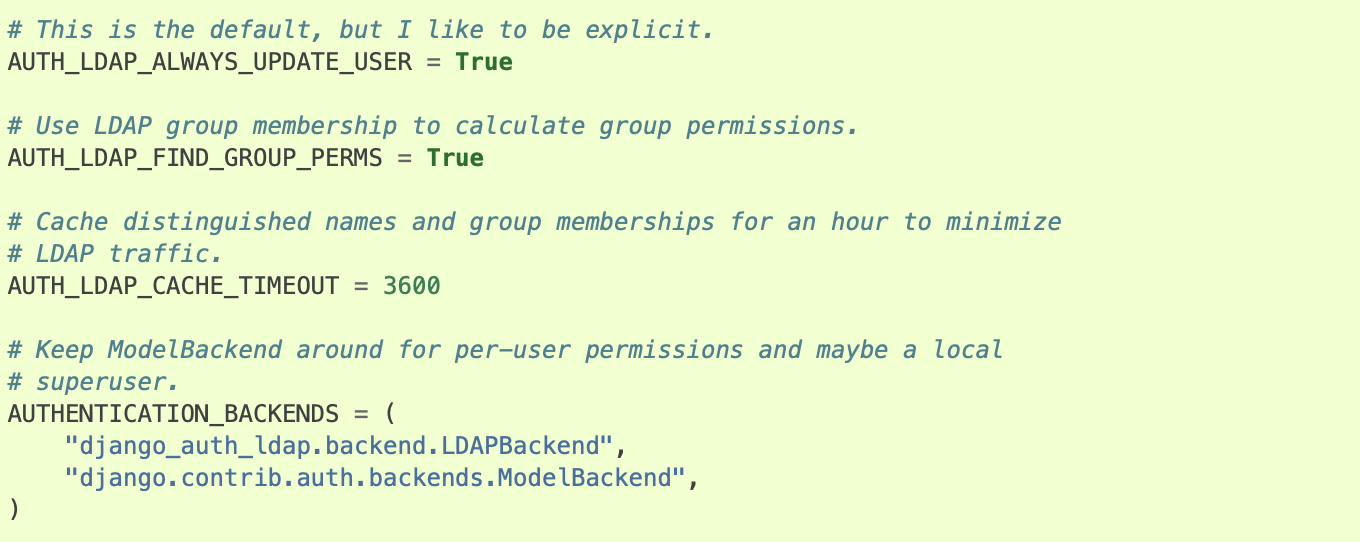
\includegraphics[width=6in]{figures/exam2}
\captionsource{Example Configuration}{\url{https://django-auth-ldap.readthedocs.io/en/latest/example.html}}
\label{figure:exam}
\end{figure}
\newpage

\section{API ที่จะนำมาเรียกใช้}
\cite{restapi}
โดย API ที่จะนำมาเรียกใช้คือ REST API สําหรับการส่งงานเขียนโปรแกรมด้วย OpenAPI และ API ที่ได้พัฒนานี้ จะรับข้อมูลคําตอบได้เฉพาะไฟล์ที่เป็นภาษาคอมพิวเตอร์ แบ่งเป็น 2 รายการดังนี้
\begin{enumerate}
    \item รายการแรกเป็น Compiler API ทําหน้าที่รับข้อมูลจากผู้ใช้และทําการตรวจสอบ
โปรแกรม โดยทําการเปรียบเทียบกับผลเฉลย และส่งผลลัพธ์กลับเป็น output
    \item API รายการที่สองเป็น Problem API สําหรับทําหน้าที่อัปเดตข้อมูลของโจทย์ปัญหาและเฉลย
\end{enumerate}

\subsection{Method ที่เซิร์ฟเวอร์ใช้ในการรับข้อมูลจากผู้ใช้}
ในการพัฒนาระบบ API ได้มีการเลือกใช้ method หลัก ๆ จํานวน 2 method คือ
method GET และ method POST โดยทั้ง 2 method มีความแตกต่างกันดังนี้
\begin{itemize}
    \item GET เป็นการดึงข้อมูลจากฐานข้อมูลของเซิร์ฟเวอร์หรือเว็บไซต์มาแสดงผลออกมาเป็น response
    \item POST เป็นการเพิ่มหรือเปลี่ยนแปลงข้อมูลต่างๆที่อยู่ในฐานข้อมูลของเซิร์ฟเวอร์เว็บไซต์
\end{itemize}
โดย API ทั้ง 2 ตัวได้มีการใช้ method ดังกล่าว ทั้ง 2 ตัวกล่าวคือ ใน Path /compile ได้มีการรองรับ
method GET และ POST และใน Path /problem ก็ได้มีการรองรับ method GET และ POST เช่น
เดียวกัน โดยได้เน้นการทํางานในส่วน method POST ดังนี้
\begin{itemize}
    \item method POST ใน /compile ทําหน้าที่รับข้อมูลเกี่ยวกับงานของนักศึกษาเพื่อนํามาประมวล
ผลและทําการแสดงคะแนนของนักศึกษาคนนั้น ๆ ที่ส่งงานหรือ assignment เข้ามาในระบบ
    \item method POST ใน /problem ทําหน้าที่รอรับ API ของผู้ที่ต้องการตรวจสอบว่า ค่า output
ของ assignment ที่ได้ทําการส่งไป มีคําตอบตรงตามที่เจ้าของ assignment เขียนไว้หรือไม่
\end{itemize}
